\documentclass[10pt, final]{article}
%\usepackage[document]{ragged2e}
\usepackage[utf8]{inputenc}

\usepackage{fancyhdr}
\setlength{\headheight}{15pt}
 
\pagestyle{fancy}
\fancyhf{}
\rhead{DFS}
\cfoot{\thepage}

\usepackage{multirow}
\usepackage{hyperref}

\usepackage{soul}

\usepackage{enumerate}
\usepackage{amssymb}
\usepackage{amsmath, mathtools}
\usepackage{amsopn}
\usepackage{amsthm}
\usepackage{color}
\usepackage{xcolor}
\usepackage{amsfonts}
\usepackage[makeroom]{cancel}
% \usepackage{wasysym}
\usepackage[paperwidth=8.5in,left=1in,right=1in,paperheight=11.0in,top=1in, bottom=1in]{geometry}

\usepackage{tikz}
\usetikzlibrary{decorations.markings}

\usepackage{pgfplots}

\pgfplotsset{compat = 1.15}
%\pgfplotsset{scaled y ticks=false}
\usetikzlibrary{positioning}
\usepackage{mathtools}

\usepackage{listings}

\DeclarePairedDelimiter\ceil{\lceil}{\rceil}
\DeclarePairedDelimiter\floor{\lfloor}{\rfloor}

\DeclareMathOperator{\im}{im}
\DeclareMathOperator{\detr}{det}
\DeclareMathOperator{\var}{var}
\DeclareMathOperator{\cov}{cov}
\DeclareMathOperator{\Real}{Re}
\DeclareMathOperator{\sgn}{sgn}
\DeclareMathOperator{\argmax}{argmax}
\DeclareMathOperator{\vect}{vec}


% Additional commands/shortcuts to make our life easier
\newcommand{\bm}{\begin{bmatrix}}
\newcommand{\fm}{\end{bmatrix}}
\def\a{\alpha}
\def\b{\beta}
\def\g{\gamma}
\def\D{\Delta}
\def\d{\delta}
\def\z{\zeta}
\def\k{\kappa}
\def\l{\lambda}
\def\n{\nu}
\def\e{\varepsilon}
\def\r{\rho}
\def\s{\sigma}
\def\S{\Sigma}
\def\t{\tau}
\def\x{\xi}
\def\w{\omega}
\def\W{\Omega}
\def\th{\theta}
\def\p{\phi}
\def\P{\Phi}
\newcommand{\pa}{\mathcal \partial}
\newcommand{\No}{\mathcal N}



\newcommand{\hatxi}{\hat{\mathbf{x}}^i}
\newcommand{\tildexi}{\tilde{\mathbf{x}}^i}



\title{Assignment 1 : DFS}
\author{Jeanne Sorin}
\date{\today}



\begin{document}

\maketitle

\section{The Model} % (fold)

% section the_model (end)

The enclosed code produces the figure below, which is a version of Figure 1 from DFS 1977, for the provided $a$ and $b$ vectors, and $g=1.0$.
\begin{figure}[h!]
	\center
	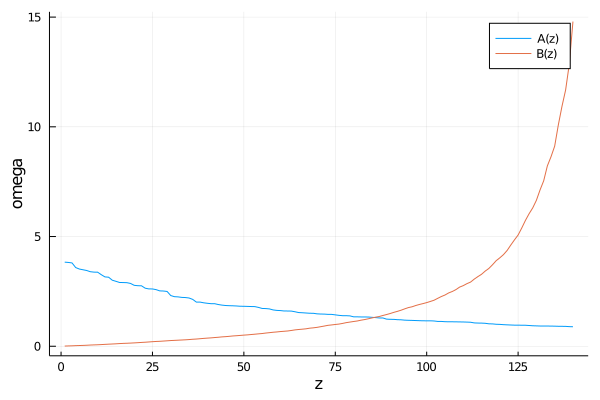
\includegraphics[width=12cm]{Fig1}
	\caption{DFS 1977 - Figure 1}
\end{figure}


\section{Gains From Trade} % (fold)
As in the lecture slides, we define welfare for Home and for Foreign as, respectively (in the discrete case)
\begin{align*}
	ln(\frac{U}{L}) &= ln(w) - \sum_{z=1}^N b(z) ln(p(z)) \\
	ln(\frac{U^*}{L^*}) &= ln(w^*) - \sum_{z=1}^N b(z) ln(p(z)^*)
\end{align*}
where $w$ ($w^*$) is wage at home (foreign), $p(z)$ ($p(z)^*$) are price levels faced at home (foreign). $b(z)$, the demand schedule, is common to both home and foreign by assumption.
\\
\\
More precisely, this implies that, for a general $g \leq 1.0$, with home importing goods $z \geq \bar{z}$ and foreign importing goods $z \leq \bar{z}^*$, normalizing $w = 1, w^* = \frac{1}{\omega}$:
\\
In autarky: $p(z) = a(z)$ and $p(z)^* = w^* a(z)^*$ and
\begin{align*}
	ln(\frac{U}{L}) &= - \sum_{z=1}^N b(z) ln(a(z)) \\
	ln(\frac{U^*}{L^*}) &= ln(\frac{1}{\omega}) - \sum_{z=1}^N b(z) ln(\frac{1}{\omega} a(z)^*)
\end{align*}
\\
Under free trade, notice that, under the general case where $g \leq 1$, we need to include transport costs in the price faced by home (foreign) on goods imported from foreign (home). Therefore, welfare under free trade is
\begin{align*}
	ln(\frac{U}{L}) &= - (\sum_{z=1}^{\bar{z}-1} b(z) ln(a(z)) + \sum_{z=1}^{\bar{z}-1} b(z) ln(\frac{a(z)^*}{\omega g}))  \\
	ln(\frac{U^*}{L^*}) &= ln(w^*) - (\sum_{z=1}^{\bar{z}^*} b(z) ln(\frac{a(z)}{g}) + \sum_{z=\bar{z}^* + 1}^N b(z) ln(\frac{a(z)^*}{\omega}))
\end{align*}
Notice that, as in the code, with $z$ is discrete, we assume that home produces on $[0,\bar{z})$ and imports on $[\bar{z}, 1]$. Similarly, foreign produces on $(\bar{z}^*, 1]$ and imports on $[0, \bar{z}^*]$.
\\
\\
The function \textit{DFS1977welfare$(a, b, L, 1.0)$} reports the following output : \\ $[1]$ gft\_home, $[2]$ gft\_foreign, $[3]$ welfare\_h (autarky), $[4]$ welfare\_home\_trade, $[5]$ welfare\_f (autarky), $[6]$ welfare\_foreign\_trade. 
\\
Running this function successively for the supplied vectors, and for a modified vector $ a^{*'} = 0.5 .* a^{*} $ representing uniform technological progress for Foreign, shows that
\begin{itemize}
	\item Both countries benefit from trade in both cases
	\item Foreign autarky welfare is higher when Foreign experiences uniform technological progress
	\item Both countries trade welfare is higher when foreign experiences uniform technological progress
	\item Gains from trade are lower for Foreign when foreign already experienced uniform technological progress in autarky
\end{itemize}

\bigskip

\noindent In addition, the \textit{DFS1977welfare} function confirms that the lower the iceberg costs (the larger $g$), the higher the gains from trade (see figure 2):
\begin{figure}[h!]
\center
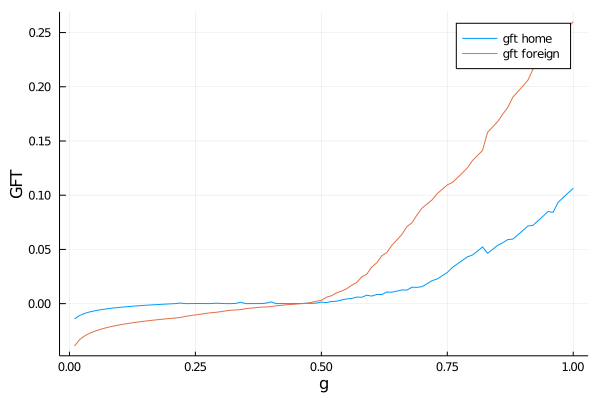
\includegraphics[width=12cm]{Fig2_WelfareGains_g}
\caption{Gains from trade as a function of iceberg costs (for provided a, b schedules)}
\end{figure}


\section{On the relationship between volume of trade and each country's gains from trade} % (fold

\textit{What is the relationship between the volume of trade and each country's gains from trade in this model? Use your solver to produce an example of different equilibria (with the same L, L*, and $g<1$) that exhibit the same volume of trade and different gains from trade. If you also hold fixed the b schedule, can you produce such an example? Why or why not? What can be said about the magnitude of the gains from trade in this model if we observe the equilibrium volume of trade and do not observe autarky prices?}
\\
\\
I show below that we can produce an example of different equilibria that exhibit the same volume of trade ($\bar{z} - \bar{z}^*$ fixed) and different gains from trade, even when holding the b schedule. Moreover, I show that we can't say much about the magnitude of the gains from trade in this model if we observe $\bar{z} - \bar{z}^*$ but not the autarky prices.
\\
\\
Let's show that multiple pairs $\bar{\omega}$ can be associated to a give $\bar{z} - \bar{z}^*$, as long as either (i) the $b(z)$ schedule or the (ii) $A(z)$ schedule is modified accordingly.
\\
From equation (19') we know that
\begin{align*}
	\bar{\omega} &= \frac{1 - \lambda^*(\bar{\omega} / g)}{1 - \lambda(g \bar{\omega})} \frac{L^*}{L} \\
	\bar{\omega} &= \frac{1 - \int_{\bar{z^*}}^1 b(z) dz}{1 - \int_0^{\bar{z}} b(z) dz} \frac{L^*}{L} \\
	\bar{\omega} &= \frac{\int_0^{\bar{z^*}} b(z) dz}{1 - \int_0^{\bar{z}} b(z) dz} \frac{L^*}{L}
\end{align*}
Moreover from equation (21)
\begin{align*}
	\bar{z}^* &= A^{-1}(\bar{\omega} / g) \\
	\bar{z} &= A^{-1}(\bar{\omega} g)
\end{align*}
Fixing the volume of trade such that, for ex, $\bar{z} - \bar{z}^* = f$
\begin{align*}
	\bar{\omega} &= \frac{\int_0^{\bar{z^*}} b(z) dz}{1 - \int_0^{\bar{z}^*} b(z) dz - \int_{\bar{z}^*}^{\bar{z}} b(z) dz} \frac{L^*}{L}
\end{align*}
Plugging into (19')
\begin{align*}
	\bar{\omega} &= \frac{\int_0^{A^{-1}(\bar{\omega} / g)} b(z) dz}{1 - \int_0^{A^{-1}(\bar{\omega} / g)} b(z) dz - \int_{A^{-1}(\bar{\omega} / g)}^{A^{-1}(\bar{\omega} g)} b(z) dz} \frac{L^*}{L}
\end{align*}
Fixing $b(z)$ and $\bar{z} - \bar{z}^*$ we can easily see from the equation above that there are multiple pairs $(\bar{\omega}, A(.))$ solving the equation, as we haven't imposed any functional form assumption on A except monotonicity. Note that, for a given $A(.)$ and $\bar{z} - \bar{z}^*$, we also have multiple pairs $(\bar{\omega}, b(z))$ solving the equation above. 
\\
\\
For the sake of simplicity, let's impose $b(z) = b, \forall z$, $L^* = L$ :
\begin{align*}
	\bar{\omega} &= \frac{A^{-1}(\bar{\omega} / g) \times b}
	{1 - A^{-1}(\bar{\omega} / g) \times b - f \times b} \\
	\bar{\omega}  - \bar{\omega} A^{-1}(\bar{\omega} / g) \times b - \bar{\omega} f \times b  &= A^{-1}(\bar{\omega} / g) \times b \\
	A^{-1}(\bar{\omega} / g) &= \bar{z}^* = \frac{\bar{\omega}(1 - f b)}{b(1 + \bar{\omega})}
\end{align*}
Intuitively, what is going on? Gains from trade are summarized by the integral between the $\bar{\omega}$ horizontal line and the $A(\bar{z})/g$ and $A(\bar{z}^*)g$ curves. Fixing $b(z) = b$ but \textit{pivoting} the A schedule such that the integrated areas are different, even though $\bar{\omega}, \bar{z}, \bar{z}^*$ are the same, will lead to different gains from trade with similar traded volumes. 
\\
\\
Alternatively, for a given A schedule, one could \textit{pivot} $b(z)$ such as to move both $\bar{z}$ and $\bar{z}^*$ such that $\bar{z} - \bar{z}^*$ is fixed, but the areas integrated are different.
\\
The figure below was obtained from solving for the equilibrium trade using the provided $A(z)$ vector, $B(z) =  1/150, \forall z$, and a modified $B'(z)$ putting more weight on lower zs (see enclosed code). Both $B$ vectors lead to the same volume of trade, but different gains from trade, for a given $A$ because $\bar{\omega} \neq \bar{\omega}'$\footnote{Generalizing this example is likely a little tricky, as what determines $\bar{z}, \bar{z}^*$ is the cumulative sum of $b(z)$ rather than its individual elements.}
\begin{figure}[h!]
\center
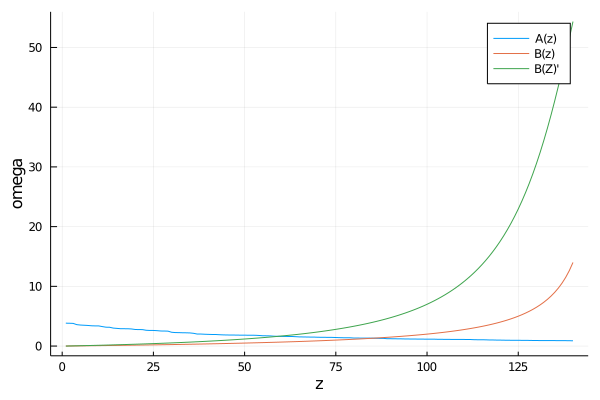
\includegraphics[width=12cm]{Fig3}
\caption{Version of Figure 1 for 2 different B schedules, leading to different $\bar{\omega}$ and therefore different gft}
\end{figure}
\\
\\
Finally, one could also think about changing A marginally such that all equilibrium quantity are unchanged $\bar{z}, \bar{z}^*, \bar{\omega}$, but the integrated areas are different. 

% section on_the_relationship_between_volume_of_trade_and_each_country_s_gains_from_trade (end)

\bigskip

\noindent Last but not least, as discussed above, observing the equilibrium volume of trade ($\bar{z} - \bar{z}^* = f$) without observing autarky prices does not allow us to say anything about the magnitude of the gains from trade in this model, as this is equivalent to not observing the $A$ schedule, and therefore not being able to estimate the integral.

% section section_name (end)


\end{document}
